% ============================================================================
% CAEM defence poster — pre-thesis-2 milestone
% Confidence-Aware Episodic Memory with Self-Improvement for Progressive
% Hallucination Reduction in Large Language Models
% CSE400 · Department of CSE · BRAC University
% Authors: Md. Aksan Gony Alif, Maliha Binte Shamim, Md. Mahmudur Rahman
% Supervisor: Dr. Md. Golam Rabiul Alam · Co-supervisor: Md. Tanzim Reza
% Built on Anish Athalye's Gemini beamerposter theme (MIT-licensed).
% Custom colour theme: beamercolorthemecaem.sty (BRAC navy + thesis figure palette).
% ============================================================================

\documentclass[final]{beamer}

% ====================
% Packages
% ====================

\usepackage[T1]{fontenc}
% luainputenc is obsolete under modern LuaTeX (UTF-8 is the native input
% encoding), so we skip it; inputenc is loaded automatically by LuaLaTeX.
\usepackage{lmodern}
\usepackage[size=custom, width=120,height=72, scale=1]{beamerposter}
\usetheme{gemini}
\usecolortheme{caem}
\usepackage{graphicx}
\usepackage{booktabs}
\usepackage{array}
\usepackage{colortbl}      % provides \rowcolor for shaded table rows
\usepackage[table]{xcolor} % colour names + table-colour support
\usepackage{tikz}
\usetikzlibrary{arrows.meta,positioning,shapes.geometric,fit,backgrounds}
\usepackage{pgfplots}
\pgfplotsset{compat=1.14}
\usepackage{anyfontsize}

% ====================
% Lengths (three-column layout: separators + columns sum to paperwidth)
% ====================

\newlength{\sepwidth}
\newlength{\colwidth}
\setlength{\sepwidth}{0.025\paperwidth}
\setlength{\colwidth}{0.3\paperwidth}

\newcommand{\separatorcolumn}{\begin{column}{\sepwidth}\end{column}}

% ====================
% Title block
% ====================

\title{CAEM: Confidence-Aware Episodic Memory with Self-Improvement}

% Authors, institute, and footer content are rendered directly by the
% overridden headline / footline templates in beamercolorthemecaem.sty.
% The previous \author / \institute / \footercontent commands have been
% removed because the BRAC Pre-Thesis 2 sample layout hardcodes the names,
% the department line, and the four footer segments inside the templates.

% ====================
% Body
% ====================

\begin{document}

\begin{frame}[t]
\begin{columns}[t]
\separatorcolumn

% ============================================================================
% COLUMN 1: the problem + the architecture + locked configuration
% ============================================================================

\begin{column}{\colwidth}

  \begin{block}{Headline result (vs.\ matched zero-shot baseline B1)}
    \textbf{Training-panel architectural-contribution slice (CAEM C2 vs.\ B1):}
    \[
      \boxed{\Delta\mathrm{EM} = +20.3\%\ \text{rel.}} \qquad
      \boxed{\Delta\mathrm{CHM} = -29.4\%\ \text{rel.}}
    \]
    Pooled training-panel EM lifts from $0.483$ at B1 to $0.581$ at CAEM C2;
    pooled training-panel CHM falls from $0.143$ to $0.101$. CAEM beats every
    one of the eight external baselines on both axes at both reference cycles
    ($8/8$ wins-against). The retrieval-utility classifier ablation lifts
    \textbf{CommonsenseQA EM by $+14.0$\,pp} and \textbf{TruthfulQA EM by
    $+10.0$\,pp} by re-routing misconception-bait queries away from the
    retrieval-augmented tier.
  \end{block}

  \begin{block}{Problem: hallucination as a deployment-safety issue}
    Modern instruction-tuned language models generate confident-sounding
    answers at deployment-relevant rates that exceed their actual accuracy
    by ten or more percentage points~[1,2]. Single-signal correctness
    predictors achieve AUROC scores between $0.50$ and $0.60$, marginally
    above chance~[3]. The TruthfulQA benchmark documents an inverse-scaling
    pattern under which larger models are \emph{more} prone to echo human
    falsehoods~[4]. Clinical-question studies report hallucination rates of
    $69$\,--\,$77\%$ on frontier models~[5].

    \heading{The three structural shortcomings}
    \begin{itemize}
      \item \textbf{Statelessness:} no representation of past verified
        answers persists across sessions.
      \item \textbf{Overconfidence:} single-signal correctness predictors
        are near random.
      \item \textbf{Immutable capability:} naive online fine-tuning
        produces catastrophic forgetting.
    \end{itemize}
    CAEM is an architectural intervention that closes all three jointly.
  \end{block}

  \begin{block}{The architecture: eight-stage pipeline + cycle-boundary loop}
    \centering
    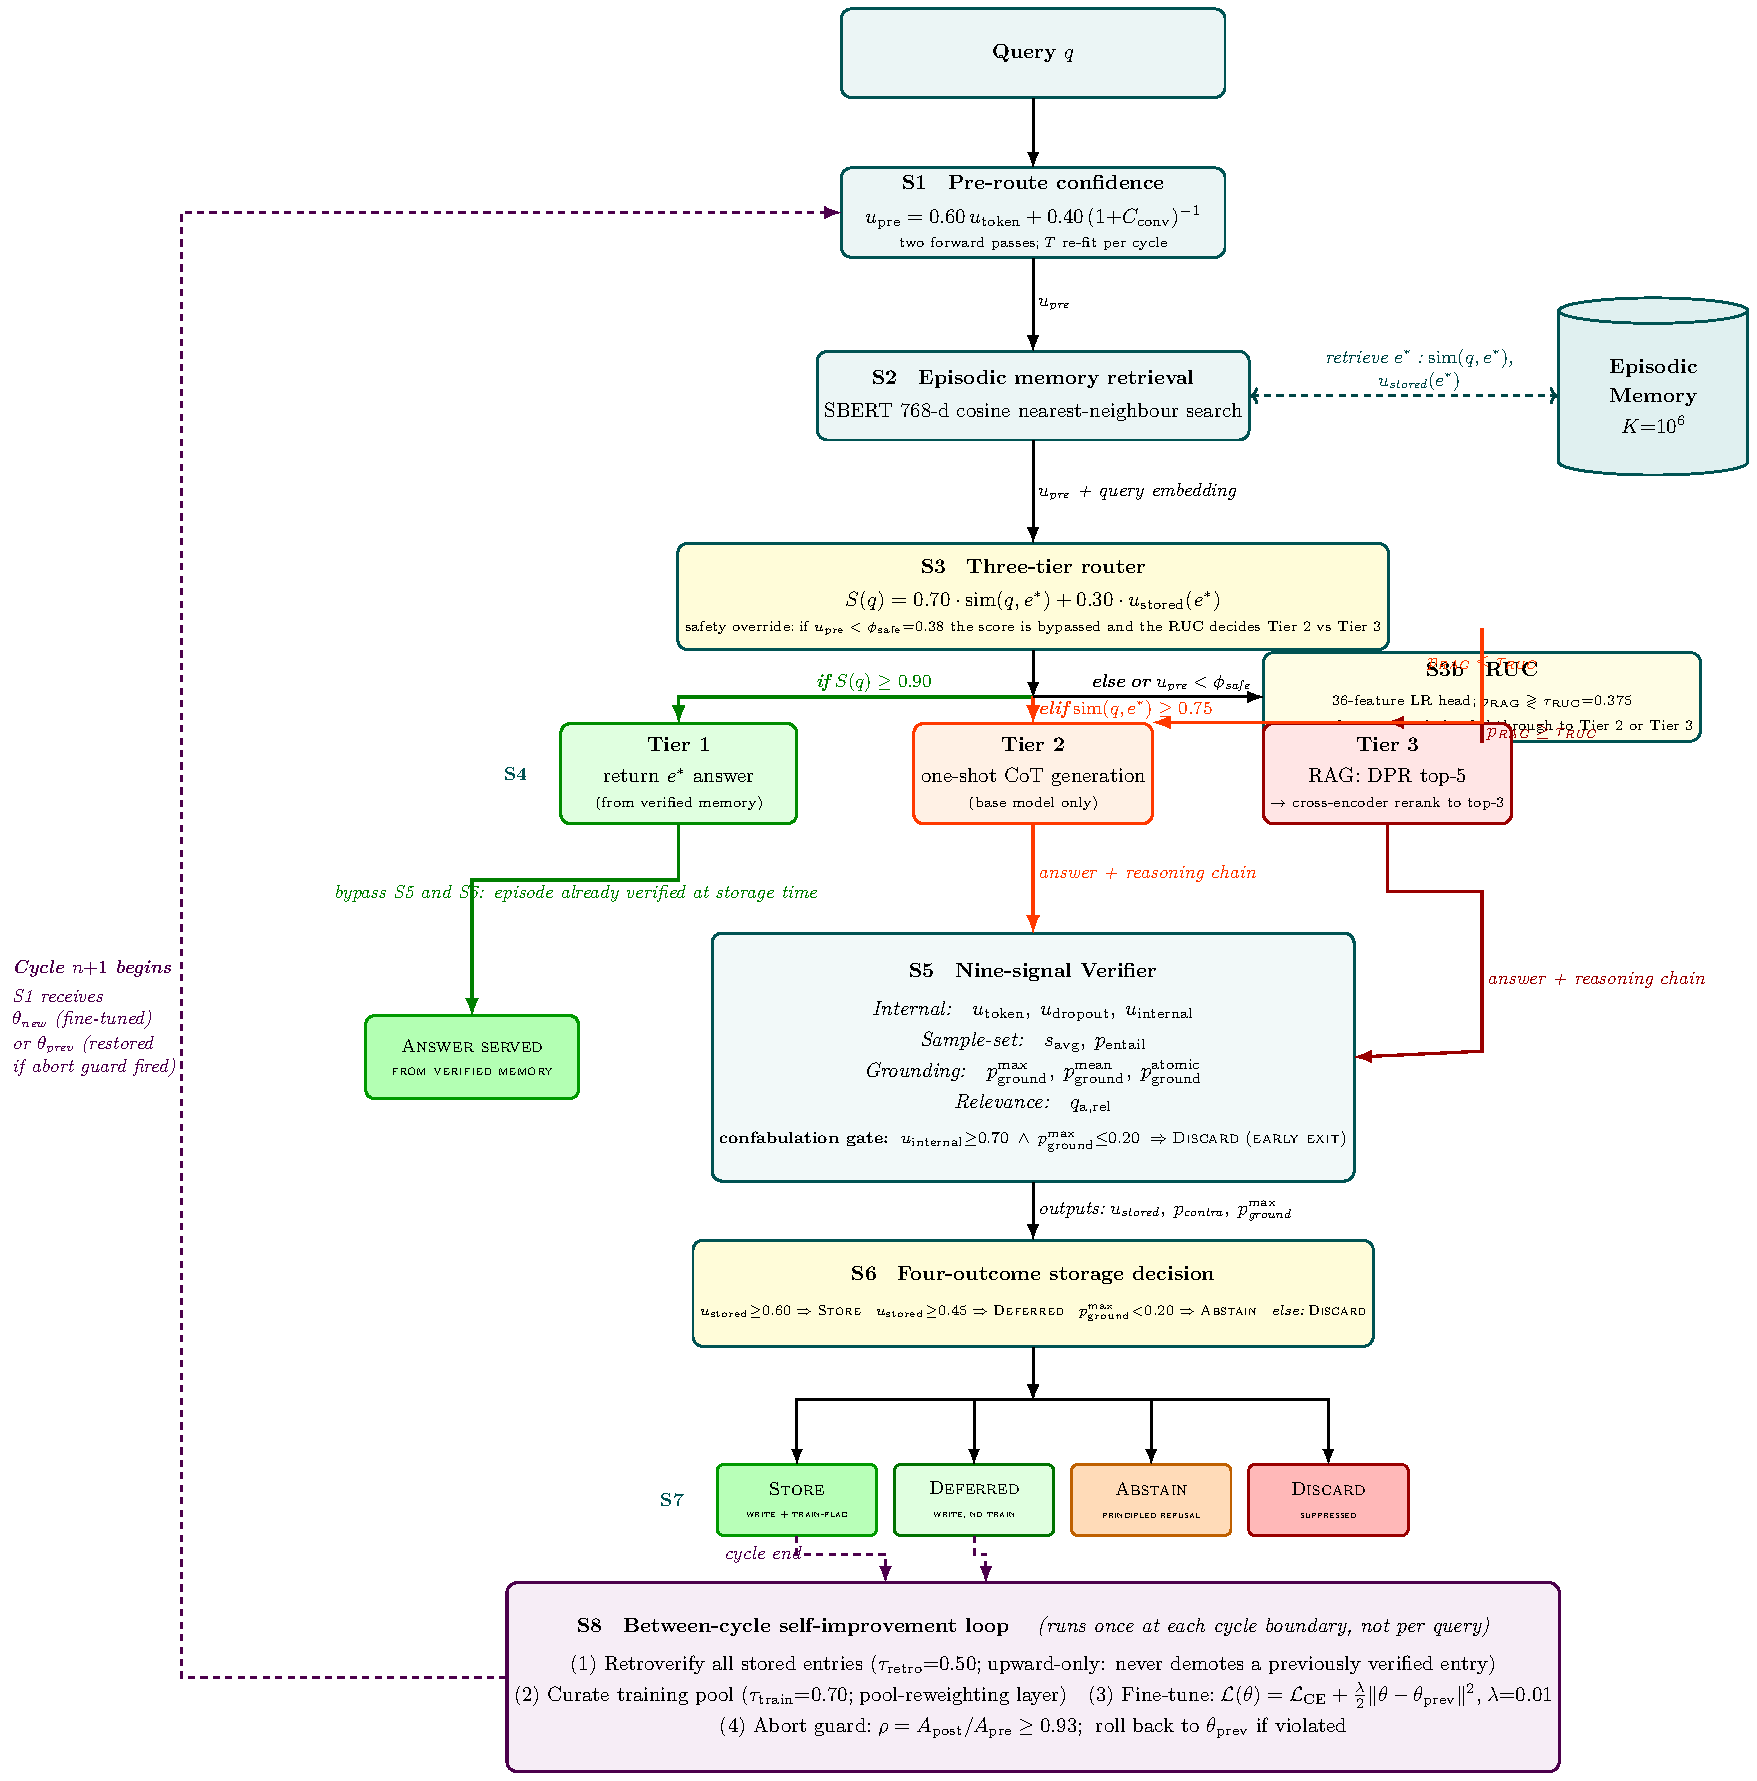
\includegraphics[width=0.98\colwidth]{figures/architecture_source.pdf}

    \vspace{0.4em}
    A query passes through pre-routing confidence, episodic memory lookup,
    three-tier dispatch, the \textbf{Stage 3b retrieval-utility classifier}
    (which intercepts the safety-override and score-formula fall-through to
    the retrieval-augmented tier), tier execution, nine-signal verification,
    the four-outcome decision tree, and output. At every committed cycle
    boundary, S8 runs the five-pass update: retroverify $\to$ deferred
    reconsider $\to$ consolidate $\to$ LoRA self-improvement fine-tune $\to$
    multi-modal retention probe (the rollback fires when the worst-probe
    ratio crosses below $\rho_{\min}=0.93$).
  \end{block}

  \begin{block}{Locked configuration (every cycle)}
    \centering
    \footnotesize
    \setlength{\tabcolsep}{8pt}
    \renewcommand{\arraystretch}{1.05}
    \begin{tabular}{@{}l l@{}}
      \toprule
      \textbf{Component} & \textbf{Value} \\
      \midrule
      Storage cut $\tau_{\text{store}}$ \,/\, $\tau_{\text{defer}}$ & $0.60$ \,/\, $0.45$ \\
      SIL admission $\tau_{\text{train}}$ & $0.70$ (strictly above $\tau_{\text{store}}$) \\
      Retroverify prune $\tau_{\text{retro}}$ & $0.50$ \\
      Retrieval-utility classifier $\tau_{\text{RUC}}$ & $0.375$ \\
      Retention floor $\rho_{\min}$ & $0.93$ on worst probe \\
      Router $\lambda$ \,/\, safety floor $\phi_{\text{pg}}$ & $0.70$ \,/\, $0.38$ \\
      Backbone & Qwen-2.5-3B-Instruct (frozen) \\
      LoRA & $r{=}32$, $\alpha{=}64$, dropout $0.05$, 7 projections \\
      Active verifier signals & $9$ ($h_{\text{norm}}$, $p_{\text{contra}}$ retired) \\
      Trajectory & registered $10$-cycle cap \,/\, realised $6$ cycles \\
      \bottomrule
    \end{tabular}
  \end{block}

\end{column}

\separatorcolumn

% ============================================================================
% COLUMN 2: methodology components + cycle-boundary trajectory
% ============================================================================

\begin{column}{\colwidth}

  \begin{block}{Nine-signal verifier $+$ calibrated probability composite}
    Four signal families feed the per-benchmark calibrated probability composite:

    \begin{itemize}
      \item \textbf{Internal calibration:} $u_{\text{token}}$, $u_{\text{dropout}}$, $u_{\text{internal}}$
      \item \textbf{Sample-set agreement:} $s_{\text{avg}}$, $p_{\text{entail}}$
      \item \textbf{External grounding:} $p_{\text{ground}}^{\max}$, $p_{\text{ground}}^{\text{mean}}$, length-gated $p_{\text{ground}}^{\text{atomic}}$
      \item \textbf{Question-answer relevance:} $q_{\text{a,rel}}$
    \end{itemize}

    \heading{Calibrated probability composite}
    Per-signal isotonic regression maps each raw signal to a calibrated
    probability; per-benchmark child curves are shrunk toward the pooled fit
    through a James-Stein-style prior at $\alpha=0.6$; an $L_2$-regularised
    logistic boost layer ($C=0.01$) aggregates the per-signal log-odds into
    $u_{\text{stored}}\in[0,1]$.

    \heading{Storage gate (fixed threshold)}
    \[
      u_{\text{stored}} \geq 0.60 \to \textsc{Store} \quad
      u_{\text{stored}} \geq 0.45 \to \textsc{Defer} \quad
      \text{else} \to \textsc{Abstain}\,/\,\textsc{Discard}
    \]
    Thresholds are frozen across cycles; only the composite refits per cycle.
    Replaces an earlier split-conformal gate rejected on the registered
    calibration-to-evaluation distribution-shift evidence.
  \end{block}

  \begin{block}{Self-improvement loop with asymmetric-rollback retention guard}
    At every committed cycle boundary:
    \begin{enumerate}
      \item \textbf{Retroverify} every stored episode under the
        \textbf{locked verifier ensemble} (MiniCheck $+$ frozen Qwen judge),
        re-scored against the updated generator's outputs and the
        cycle-boundary-refit composite. Prune entries that fall below
        $\tau_{\text{retro}}=0.50$.
      \item \textbf{Reconsider} every entry in the deferred buffer
        (promote, drop, keep) under TTL $=2$ cycles.
      \item \textbf{Consolidate} near-duplicate-meaning clusters under a
        cosine-similarity floor of $0.92$.
      \item \textbf{Fine-tune} the LoRA adapter on the strict training pool
        ($\tau_{\text{train}}=0.70$); three epochs, effective batch $16$.
      \item \textbf{Probe} the registered multi-modal retention panel (MMLU,
        TQA-test, CSQA-test). If the worst-probe ratio drops below
        $\rho_{\min}=0.93$, the adapter rolls back to the previous committed
        checkpoint while \textbf{the memory store is preserved across the
        rollback} (the asymmetric-rollback contract).
    \end{enumerate}
    Crucially, only the \emph{generator} (advancing via SIL) and the
    \emph{composite} (refitting per cycle) are cycle-indexed; the verifier
    ensemble is held fixed by design, so the per-cycle cal-fold class
    separation is a joint observable of the SIL-advanced generator viewed
    through that fixed lens.
  \end{block}

  \begin{block}{Cycle-boundary trajectory: SIL $+$ memory $+$ commit pattern}
    \centering
    \footnotesize
    \setlength{\tabcolsep}{6pt}
    \renewcommand{\arraystretch}{1.05}
    \begin{tabular}{@{}l r r r c r@{}}
      \toprule
      \textbf{Cycle} & \textbf{SIL\,$n$} & \textbf{Final loss} & \textbf{Worst probe} & \textbf{Commit} & \textbf{Memory pool} \\
      \midrule
      C1 & $107$    & $0.258$ & $1.006$            & $\checkmark$ & $2\,818$ \\
      C2 $\star$ & $1\,474$ & $0.171$ & $0.949$    & $\checkmark$ & $5\,151$ \\
      C3 & $2\,966$ & $0.109$ & $0.976$            & $\checkmark$ & $7\,477$ \\
      C4 & $3\,624$ & $0.070$ & $\mathbf{0.886}$   & $\times$ \textbf{ABORT} & $9\,961$ \\
      C5 & $5\,006$ & $0.091$ & $0.958$            & $\checkmark$ & $\mathbf{12\,175}$ \\
      \bottomrule
    \end{tabular}

    \vspace{0.4em}
    The realised commit pattern $(1,1,1,0,1)$ yields commit fraction
    $\widehat{\pi}_{\text{commit}}=4/5=0.80$, strictly in the open interval
    $(0, 1)$. The memory pool grows monotonically from $431$ cold-start
    entries to $12\,175$ at the cycle-five close \textbf{even across the
    cycle-four retention abort}, because the stream-chunk path executes
    independently of the retention guard under the asymmetric-rollback
    contract: deployment-time cost amortisation (memory tier growth)
    decouples from training-time parametric progression (adapter commits).
    Final-cycle losses decline monotonically across the four uninterrupted
    fine-tunes ($0.258 \to 0.171 \to 0.109 \to 0.070$), the empirical
    receipt that SIL makes coherent gradient progress on the verified pool.
  \end{block}

\end{column}

\separatorcolumn

% ============================================================================
% COLUMN 3: empirical results (headline + baseline panel + per-cycle trajectory)
% ============================================================================

\begin{column}{\colwidth}

  \begin{block}{Per-cycle pooled trajectory (5-benchmark evaluation panel)}
    \centering
    \footnotesize
    \setlength{\tabcolsep}{6pt}
    \renewcommand{\arraystretch}{1.05}
    \begin{tabular}{@{}l r r c c c@{}}
      \toprule
      \textbf{Cycle} & \textbf{Pooled EM} & \textbf{Pooled CHM} & \textbf{MMLU} & \textbf{TQA-test} & \textbf{CSQA-test} \\
      \midrule
      \rowcolor{lightgrey} B1 (zero-shot ref) & $0.507$ & $0.120$ & \,---\, & \,---\, & \,---\, \\
      C0 & $0.541$ & $0.135$ & \,---\, & \,---\, & \,---\, \\
      C1 & $0.543$ & $0.112$ & $1.041$ & $1.013$ & $1.006$ \\
      \rowcolor{caemTealLight}
      \textbf{C2 $\star$} & $\mathbf{0.544}$ & $\mathbf{0.107}$ & $0.975$ & $0.949$ & $0.982$ \\
      C3 & $0.532$ & $0.115$ & $0.992$ & $0.987$ & $0.976$ \\
      \rowcolor{caemRedLight}
      C4 \textbf{abort} & $0.532$ & $0.115$ & $1.018$ & $\mathbf{0.886}$ & $0.982$ \\
      C5 (final) & $0.517$ & $0.109$ & $0.999$ & $1.013$ & $0.958$ \\
      \bottomrule
    \end{tabular}

    \vspace{0.4em}
    \footnotesize
    The composite hallucination metric reduces $-19\%$ relative across the
    trajectory and attains its minimum at C2. C4 fires the retention guard
    on TQA-test $=0.886 < \rho_{\min}=0.93$; C5 recovers to $0.958$. Pool
    purity holds in the band $[0.732, 0.746]$ on the cal fold across all
    committed cycles, clearing the registered $0.64$ floor by $9$\,--\,$11$\,pp.
  \end{block}

  \begin{block}{External eight-baseline panel (matched protocol)}
    \centering
    \footnotesize
    \setlength{\tabcolsep}{4pt}
    \renewcommand{\arraystretch}{1.05}
    \begin{tabular}{@{}l l r r r r@{}}
      \toprule
      & \textbf{System} & \textbf{EM} & \textbf{CHM} & $\boldsymbol{\Delta}$\textbf{EM} & $\boldsymbol{\Delta}$\textbf{CHM} \\
      & & & & \textbf{vs C2} & \textbf{vs C2} \\
      \midrule
      \rowcolor{caemTealLight}
      $\star$ & \textbf{CAEM C2 (best)} & $\mathbf{0.544}$ & $\mathbf{0.107}$ & --- & --- \\
              & CAEM C5 (final) & $0.517$ & $0.109$ & $-0.027$ & $+0.002$ \\
      \midrule
      B1 & zero-shot & $0.507$ & $0.120$ & $+7.4\%$ & $-11.0\%$ \\
      B2 & chain-of-thought & $0.500$ & $0.123$ & $+8.8\%$ & $-12.7\%$ \\
      B3 & DPR-RAG & $0.458$ & $0.148$ & $+18.8\%$ & $-27.7\%$ \\
      B4 & CoT $+$ DPR-RAG & $0.461$ & $0.142$ & $+17.9\%$ & $-24.6\%$ \\
      B5 & five-shot CoT & $0.405$ & $0.136$ & $+34.2\%$ & $-21.4\%$ \\
      B6 & vanilla fine-tune (C5) & $0.325$ & $0.144$ & $+67.2\%$ & $-25.5\%$ \\
      B7 & FLARE & $0.292$ & $0.153$ & $+86.3\%$ & $-29.9\%$ \\
      B8 & semantic entropy & $0.505$ & $0.120$ & $+7.7\%$ & $-10.5\%$ \\
      \bottomrule
    \end{tabular}

    \vspace{0.4em}
    \footnotesize
    \textbf{Wins-against: CAEM C2 beats $8/8$ baselines; CAEM C5 beats $8/8$.}
    CHM is post-hoc rescored through the locked CAEM verifier for every row,
    so the column is apples-to-apples. TruthfulQA EM uses the Haiku-judged
    correctness rule for every row including the abstention-licensed B8.
  \end{block}

  \begin{block}{Retrieval-utility-classifier ablation (C3 close)}
    \centering
    \footnotesize
    \setlength{\tabcolsep}{4pt}
    \renewcommand{\arraystretch}{1.05}
    \begin{tabular}{@{}l c c c c c c@{}}
      \toprule
      \textbf{Benchmark} & \textbf{EM off} & \textbf{EM on} & $\boldsymbol{\Delta}$\textbf{EM (pp)} & \textbf{T3 share off} & \textbf{T3 share on} & $\boldsymbol{\Delta}$ \\
      \midrule
      FEVER          & $0.503$ & $0.503$ & $0.0$            & $92.3\%$ & $70.7\%$ & $-21.7$ \\
      TriviaQA       & $0.437$ & $0.463$ & $+2.7$           & $95.7\%$ & $68.0\%$ & $-27.7$ \\
      \rowcolor{caemOrangeLight}
      \textbf{CommonsenseQA}  & $0.603$ & $\mathbf{0.743}$ & $\mathbf{+14.0}$ & $57.7\%$ & $20.3\%$ & $-37.3$ \\
      StrategyQA     & $0.617$ & $0.640$ & $+2.3$           & $100.0\%$ & $76.7\%$ & $-23.3$ \\
      \rowcolor{caemOrangeLight}
      \textbf{TruthfulQA}     & $0.210$ & $\mathbf{0.310}$ & $\mathbf{+10.0}$ & $99.0\%$ & $40.0\%$ & $\mathbf{-59.0}$ \\
      \midrule
      \textbf{Pooled} & $\mathbf{0.474}$ & $\mathbf{0.532}$ & $\mathbf{+5.8}$ & $\mathbf{88.9\%}$ & $\mathbf{55.1\%}$ & $\mathbf{-33.8}$ \\
      \bottomrule
    \end{tabular}

    \vspace{0.4em}
    \footnotesize
    The asymmetric-rescue pattern (bold cells): the largest EM gains land
    on CommonsenseQA and TruthfulQA, the two benchmarks where retrieval was
    actively hurting in the classifier-off arm. FEVER EM stays flat: the
    classifier correctly preserves the retrieval-helpful regime on a
    textbook fact-verification benchmark.
  \end{block}

  \begin{block}{Code, data, and references}
    \footnotesize
    \textbf{Code:} \texttt{github.com/aksaN000/caem-thesis}\quad
    \textbf{Artefacts (Google Drive):} \texttt{drive.google.com/drive/folders/} \texttt{1xErhsRDYe\_qO0ZgUBn0WXK81eHc5jZCa} \quad
    \textbf{Passage index (HF, private):} \texttt{aksaN000/caem-passage-index-21m}

    \vspace{0.5em}
    \scriptsize
    {[1]} Guo et al., \emph{ICML 2017}. \,
    {[2]} Kadavath et al., \emph{arXiv 2022}. \,
    {[3]} Xiong et al., \emph{ICLR 2024}. \,
    {[4]} Lin et al., \emph{ACL 2022}. \,
    {[5]} Alkaissi \& McFarlane, \emph{Cureus 2023}. \,
    {[6]} Thorne et al., \emph{NAACL 2018}. \,
    {[7]} Joshi et al., \emph{ACL 2017}. \,
    {[8]} Talmor et al., \emph{NAACL 2019}. \,
    {[9]} Geva et al., \emph{TACL 2021}. \,
    {[10]} Hu et al., \emph{ICLR 2022} (LoRA). \,
    {[11]} Tang et al., \emph{2024} (MiniCheck). \,
    {[12]} Cherian et al., \emph{2024} (boost layer).
  \end{block}

\end{column}

\separatorcolumn
\end{columns}
\end{frame}

\end{document}
